\chapter{ ГЛАВА 3. Реализация модели в Timefold Solver}
\label{ch:chapter3}

\section{Архитектура и ключевые понятия Timefold Solver}

Для реализации задачи оптимизации выбрана библиотека Timefold Solver — современный инструмент для решения задач планирования и расписания с использованием эвристик и метаэвристик. Timefold позволяет описывать модель задачи через аннотированные Java-классы и автоматически подбирать эффективную стратегию поиска решения.

Он используется для:
\begin{itemize}
    \item Производственного планирования.
    \item Расписаний.
    \item Логистики.
    \item фасовки продуктов
\end{itemize}

Общий процесс планирования сводится к нескольким этапам.

Моделирование задачи. В данный процесс входят описание сущности @PlanningEntity, назначение переменных @PlanningVariable, определение решения @PlanningSolution, после чего задаются ограничения ConstraintProvider.

Инициализация решателя. Читает конфигурацию из XML или Java DSL. Загружает решение и возможные значения переменных.

Фаза Construction Heuristics. Быстро создаёт первое допустимое решение. Например, назначает задания на любые линии с минимальными нарушениями.

Фаза Local Search. Итеративно улучшает решение с помощью эвристик: Late Acceptance, Simulated Annealing, Tabu Search, Great Deluge. На каждом шаге: применяет ход $\rightarrow$ пересчитывает score $\rightarrow$ решает, принимать ли новое решение.
 
По достижении времени/шага/качества решение сохраняется. Может быть просмотрено в приложении, сохранено в БД или отправлено пользователя.

Основные аннотацииями являются:

\begin{enumerate}
    \item @PlanningSolution
    \item @PlanningEntity
    \item @PlanningVariable
    \item ValueRangeProvider
    \item @ShadowVariable
    \item @CascadingShadowVariable
    \item @ProblemFact и @ProblemFactCollectionProperty
\end{enumerate}

@PlanningSolution. Аннотирует корневой класс, содержащий всё решение.

@PlanningEntity. Аннотирует объекты, чьи поля (переменные) изменяются при решении задачи.

@PlanningVariable. Указывает на переменную, которую решатель будет оптимизировать. Аргументы: valueRangeProviderRefs — имя метода или поля, дающего допустимые значения.

ValueRangeProvider. Объявляет допустимые значения для @PlanningVariable.

@ProblemFact и @ProblemFactCollectionProperty. Описывают неизменяемые факты (например, список линий, типов продуктов), которые используются при расчётах и ограничениях.

@ShadowVariable. Переменная, автоматически вычисляемая на основе других переменных. Примеры:
        \begin{itemize}
            \item endTime = startTime + duration
            \item duration = quantity / speed, где speed зависит от линии
        \end{itemize}

CascadingShadowVariable. Обозначает, что при изменении переменной также должны быть обновлены зависимые shadow-поля.

\section{Как работает планировщик}
 В данной модели основные объекты, изменяемые в процессе поиска решения и помеченные аннотацией @PlanningEntity являются классы Job и Line. Оба они играют ключевую роль в формировании расписания. \

 Класс Job — производственный заказ.

 Job представляет собой конкретное производственное задание: упаковку определённого количества конкретного продукта на одной из линий. Этот класс является основной единицей планирования, которую необходимо распределить по линиям и во времени. \

 \vspace{5cm}

 \begin{lstlisting}[caption={класс Job}, label={lst:classJob}]
@PlanningEntity
public class Job {

    @PlanningId
    private String id;
    private String name;
    private Product product;
    private int quantity;
    private Duration duration;
    private LocalDateTime minStartTime;
    private LocalDateTime idealEndTime;
    private LocalDateTime maxEndTime;
    private int priority;
    @PlanningPin
    private boolean pinned;

    ...
}
\end{lstlisting}

 Основные свойства. 

Идентификатор и имя задания (id, name) — уникальные строки для идентификации.

Продукт (product) — экземпляр класса Product, указывающий, что упаковывается.

Количество и длительность (quantity, duration) — определяют объём работы и необходимое время.

Ограничения по времени (minStartTime, idealEndTime, maxEndTime) — задают временные рамки.

Приоритет (priority) — влияет на предпочтение раннего выполнения.

Флаг pinned (@PlanningPin) — фиксирует задание, запрещая перемещение во время планирования.

Текущая линия (line) — ссылка на Line, где выполняется задача.

Цепочка соседних задач (previousJob, nextJob) — формируют последовательность выполнения.

Расчётные времена (startCleaningDateTime, startProductionDateTime, endDateTime) — вычисляются автоматически при изменении позиции задания в цепочке.

 С помощью аннотации @CascadingUpdateShadowVariable реализуется автоматическое обновление временных характеристик при изменении порядка заданий или линии. Метод updateStartCleaningDateTime() учитывает:
 \begin{enumerate}
    \item конец предыдущего задания на линии;
    \item длительность мойки между двумя типами продуктов;
    \item длительность самого задачи.
 \end{enumerate}

 Job — это основной объект, который перемещается по временной оси и между линиями. Планировщик изменяет его назначение (line) и его позицию в последовательности (через список jobs в Line).
 
Класс Line — фасовочная линия. Представляет линию, на которую назначаются задачи. Каждая линия имеет уникальный идентификатор, оператора и момент начала работы.

\begin{lstlisting}[caption={класс Line}, label={lst:classLine}]
@PlanningEntity
public class Line {

    @PlanningId
    private String id;
    private String name;
    private String operator;
    private LocalDateTime startDateTime;

    @JsonIgnore
    @PlanningListVariable
    private List<Job> jobs;
    ...
}
\end{lstlisting}

Основные свойства:

\begin{enumerate}
    \item Идентификатор, имя и оператор (id, name, operator) — идентификация линии.
    \item Время начала (startDateTime) — определяет первую возможную дату запуска заданий.
    \item Список задач (@PlanningListVariable List<Job> jobs) — определяет последовательность выполнения заданий на линии.
\end{enumerate}

Почему Line — @PlanningEntity.

Хотя сам объект Line не изменяется во время решения, он содержит список Job, аннотированный @PlanningListVariable. Это означает, что Timefold будет распределять Job по разным Line и формировать порядок заданий внутри каждой линии. Таким образом, именно список jobs внутри Line является переменной планирования. Это позволяет использовать так называемую chain-based модель планирования: задания образуют связанный список (chain), где порядок имеет значение, и каждый элемент ссылается на предыдущий и следующий через @PreviousElementShadowVariable и @NextElementShadowVariable. \

Класс PackagingSchedule представляет собой основную модель планирования, помеченную аннотацией @PlanningSolution, что означает, что именно этот класс Timefold Solver будет использовать как решаемую задачу (solution). Он содержит все необходимые данные для построения и оценки расписания фасовки продукции, включая как факты проблемы, так и планируемые сущности.

\begin{lstlisting}[caption={класс PackagingSchedule}, label={lst:classPackagingShedule}]
@PlanningSolution
public class PackagingSchedule {

    @ProblemFactProperty
    private WorkCalendar workCalendar;

    @ProblemFactCollectionProperty
    private List<Product> products;

    @PlanningEntityCollectionProperty
    private List<Line> lines;

    @PlanningEntityCollectionProperty
    @ValueRangeProvider
    private List<Job> jobs;

    @PlanningScore
    private HardMediumSoftLongScore score;

    // Ignored by Timefold, used by the UI to display solve or stop solving button
    private SolverStatus solverStatus;
    ...
}
\end{lstlisting}


Основные элементы:

\begin{itemize}
    \item @ProblemFactProperty workCalendar
    \item @ProblemFactCollectionProperty products
    \item @PlanningEntityCollectionProperty lines
    \item @PlanningScore score
    \item solverStatus
\end{itemize}

@ProblemFactProperty workCalendar. Представляет рабочий календарь — ограничение по начальной и конечной дате производственного цикла. Это неизменяемый факт, влияющий на планирование.

@ProblemFactCollectionProperty products. Список всех продуктов, которые необходимо учитывать при планировании (например, их тип, наличие аллергенов, глазурь и т.д.). Это тоже входные данные, не подлежащие изменению в процессе решения.

@PlanningEntityCollectionProperty lines. Список фасовочных линий. Несмотря на то что линии сами по себе не изменяются, они могут быть аннотированы как @PlanningEntity, если содержат переменные, которые меняются во время решения (например, последовательность заданий).

@PlanningEntityCollectionProperty и @ValueRangeProvider jobs. Список заданий (Job), которые нужно распределить между фасовочными линиями и во времени. Это главные планируемые объекты, которые Solver будет изменять в поисках оптимального решения. Аннотация @ValueRangeProvider означает, что значения из этого списка могут быть использованы в качестве допустимых значений для переменных других сущностей (например, Line).

@PlanningScore score. Поле для хранения итоговой оценки решения. Используется тип HardMediumSoftLongScore, который включает:
    \begin{itemize}
        \item жёсткие ограничения (hard): например, пересечение заданий по времени на одной линии;
        \item средние ограничения (medium): например, соблюдение приоритетов заданий;
        \item мягкие ограничения (soft): например, минимизация времени простоев и мойки.
    \end{itemize}

Поле solverStatus (не аннотировано). Не используется самим планировщиком Timefold, но необходимо для отображения текущего статуса решения в пользовательском интерфейсе (например, на фронтенде Quarkus-приложения).

Класс PackagingSchedule служит связующим звеном между:
\begin{enumerate}
    \item входными данными, загружаемыми из производственной базы данных MES;
    \item логикой планирования, реализованной в ConstraintProvider;
    \item пользовательским интерфейсом, отображающим расписание в веб-приложении на Quarkus.
\end{enumerate}

Во время запуска планировщик Timefold изменяет переменные планирования внутри объектов Job, стараясь минимизировать оценочную функцию (score) с учётом всех введённых ограничений.

\section{Ограничения и ConstraintProvider}

Ограничения (constraints) — это основа работы планировщика Timefold Solver. Они определяют, какие решения считаются допустимыми (жёсткие ограничения) и какие — предпочтительными (мягкие ограничения). Реализация ограничений выполняется в классе, реализующем интерфейс ConstraintProvider.

В данной работе используется класс FoodPackagingConstraintProvider, реализующий интерфейс ConstraintProvider. Метод defineConstraints возвращает массив всех ограничений, разделённых по уровням важности: hard, medium и soft. Оценка расписания производится с использованием трёхуровневого скоринга HardMediumSoftLongScore.

\begin{lstlisting}[caption={класс FoodPackagingConstraintProvider}, label={lst:classConstraintProvider}]
public class FoodPackagingConstraintProvider implements ConstraintProvider {

    @Override
    public Constraint[] defineConstraints(ConstraintFactory factory) {
        return new Constraint[] {
                // Hard constraints
                maxEndDateTime(factory),
                plushMustBeOnLine1(factory),
                rodOnlyOnLines456(factory),
                cactusOnlyOnLines123(factory),
                classicOnlyOnLines1236(factory),
                // Medium constraints
                idealEndDateTime(factory),
                // Soft constraints
                operatorCleaningConflict(factory),
                minimizeMakespan(factory)
        };
    }
    ...
}
\end{lstlisting}

Жёсткие ограничения (Hard constraints) обязательно должны соблюдаться. Нарушение любого из них делает решение недопустимым.

\begin{itemize}
    \item maxEndDateTime — запрещает завершать работу позже максимально допустимого времени. Штраф пропорционален количеству минут просрочки.
    \item plushMustBeOnLine1 — продукция типа PLUSH может быть упакована только на линии 1.
    \item rodOnlyOnLines456 — продукция типа ROD может быть фасована только на линиях 4, 5 или 6.
    \item cactusOnlyOnLines123 — продукция типа CACTUS допускается к фасовке только на линиях 1, 2 или 3.
    \item classicOnlyOnLines1236 — продукция типа CLASSIC допускается к фасовке только на линиях 1, 2, 3 и 6.
\end{itemize}

Эти ограничения учитывают как бизнес-правила, так и технологические особенности фасовочных линий.

Ограничения средней важности (Medium constraints) влияют на качество решения, но не делают его недопустимым при нарушении. Пример:

idealEndDateTime — желательно, чтобы задание завершилось не позже «идеального» времени (idealEndTime). При нарушении начисляется штраф, пропорциональный количеству минут отклонения.

Это ограничение даёт планировщику гибкость в пределах допустимого окна, улучшая соблюдение предпочтительных сроков.

 Мягкие ограничения (Soft constraints) направлены на улучшение качества решения с точки зрения эффективности и удобства. Пример:

 operatorCleaningConflict — минимизирует конфликты в расписании мойки между заданиями, закреплёнными за одним оператором. Если два задания требуют внимания одного оператора и пересекаются во времени, начисляется штраф за пересечение интервалов между startCleaningDateTime и startProductionDateTime.

 minimizeMakespan — минимизирует общую продолжительность работы линии. Рассчитывается как квадрат времени от начала смены до завершения последнего задания. Это способствует равномерному распределению нагрузки и завершению смен вовремя.

 minimizeCleaningDuration (пока не включено в массив ограничений) — штрафует за чрезмерную длительность промежутков между заданиями, возникающих из-за необходимости санитарной обработки (мойки). Чем выше приоритет задания, тем выше штраф за долгую подготовку к его производству.

 Взаимодействие ограничений.

Ограничения организованы по трём уровням важности, что позволяет Timefold Solver эффективно искать компромиссы:

\begin{itemize}
    \item Нарушения жёстких ограничений полностью исключают решение;
    \item Средние ограничения помогают расставить приоритеты внутри допустимых решений;
    \item Мягкие ограничения способствуют повышению эффективности, снижению издержек и упрощению логистики.
\end{itemize}

Использование Constraint Streams позволяет выразить ограничения декларативно, а не императивно, что упрощает понимание и расширение модели.
\section{Визуализация расписания фасовки с Timefold и Quarkus}

Для наглядного представления результатов оптимизации используется встроенная визуализация, предоставляемая Timefold Solver. Эта визуализация позволяет в режиме реального времени наблюдать, как выполняется планирование, и какие изменения происходят в расписании при пересчёте.

Визуализация интегрирована в веб-приложение на Quarkus. Она использует @QuarkusApplication и @ApplicationScoped для управления жизненным циклом,загружает демонстрационные данные из базы данных MES с помощью JDBC и сохраняет их в планировочную сущность PackagingSchedule предоставляет REST-интерфейсы и WebSocket, к которым подключается встроенная фронтенд-визуализация Timefold.

Цикл работы визуализации.

При запуске приложение загружает производственный заказ из SQL-базы. Вызов repository.write(solution) сохраняет начальную версию PackagingSchedule в базу данных и инициирует планирование. Далее Timefold запускает решение и отображает его во встроенном графическом интерфейсе. После чего пользователь может наблюдать цепочки заданий, их распределение по линиям и временные интервалы, сравнивать разные планы и видеть ограничения.

 Пример компонентов визуализации:

 \begin{itemize}
    \item Jobs (Задачи): визуализируются как прямоугольники на временной шкале.
    \item Lines (Линии): каждая линия — отдельный горизонтальный ряд.
    \item Cleaning time (Мойка): отображается в виде пауз между заданиями.
    \item Constraints: могут быть подсвечены при нарушении (например, слишком короткое время между аллергенами).
 \end{itemize}

 \begin{figure}[ht]
 \centering
		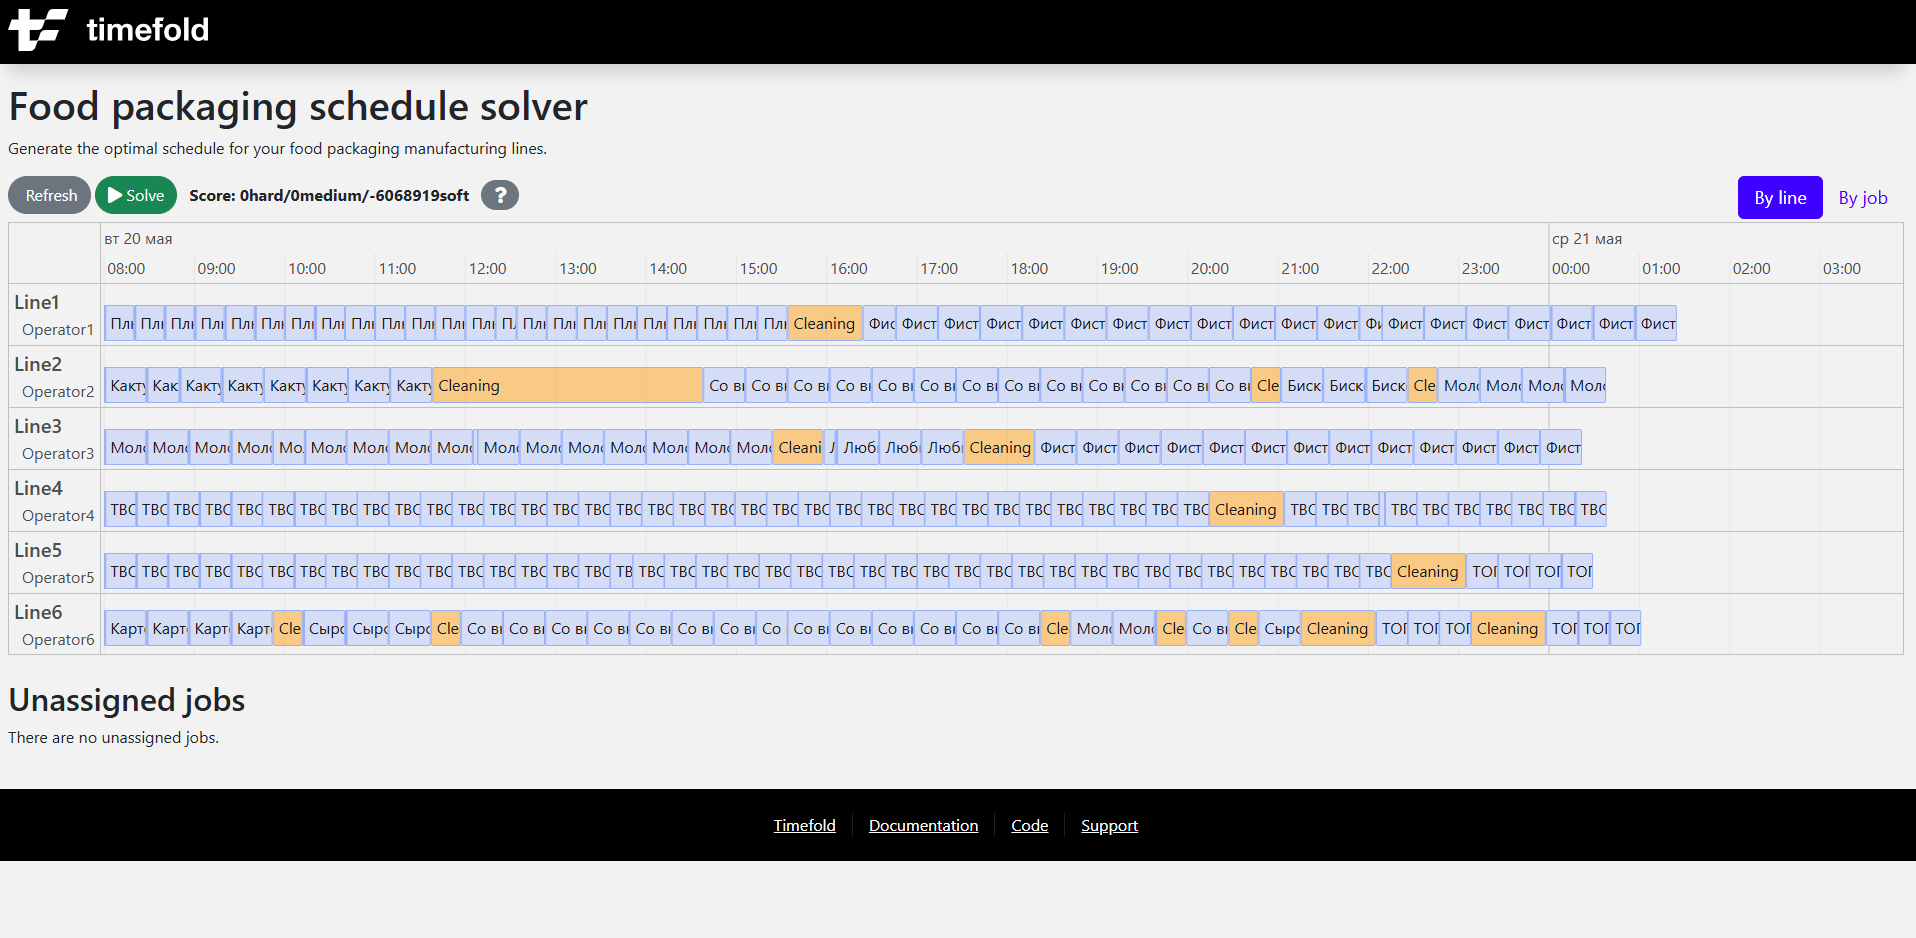
\includegraphics[height = 8 cm, keepaspectratio]{../assets/images/3_1_1Quarkus.png}
		\caption{Визуализация расписания планирования}
		\label{fig:diagram_1}
\end{figure}

